\chapter{Background}

\section{Distributed Systems}

Distributed systems are a computing paradigm characterized by independence of computational units and no universal clock.
Components in a distributed system may not directly share computational resources or memory.
Instead, computers in a distributed system typically interact through a message passing interface.

As a result, distributed computing is a challenging area of research.
In a distributed system, since processes do not share a universal clock, the ordering of messages and events needed to be carefully considered to ensure correct operation of the system.
Additionally, since individual components fail, determining which components fail and how they affect the system as a whole is also difficult in a distributed system.
Different types of failures can cause different kinds of information to be withheld or changed, disrupting those processes.

\section{Execution And Communication Models}

In this work we consider a distributed system where no processes in the system share an address space.
All processes must use a message passing interface in order to communicate with other processes to exchange information.
As a result of the complexities of distributed systems, various execution models have been developed to define how the execution of a distributed system proceeds.
Different execution models affect how easy it is to reason about the system's execution, the types of algorithms that can be executed, and how complicated they are to implement.

\subsection{Communication Channels}
We describe the avenues of communication between processes as channels.
A channel is classified as reliable if it meets 3 axioms:

\begin{axm}
    \label{axm:reliable-channel-sender}
    Every message sent by a sender is received by a receiver and every received message was sent by a sender in the system. \cite{DISTRIBUTED}
\end{axm}

\begin{axm}
    \label{axm:reliable-channel-delay}
    Every message has an arbitrary but not infinite propagation delay.\cite{DISTRIBUTED}
\end{axm}

\begin{axm}
    \label{axm:reliable-channel-fifo}
    Every channel is a \ac{FIFO} channel. If process $P$ sends a messages $x$ and $y$ to $Q$ (in that order) then $Q$ receives the messages in order ($x$ then $y$).\cite{DISTRIBUTED}
\end{axm}

These are often referred to as synchronous channels.
In this work, however, channels are not assumed to be perfectly reliable.
Instead, we respect Axiom \ref{axm:reliable-channel-fifo}, partially fulfill Axiom \ref{axm:reliable-channel-sender}, and disregard Axiom \ref{axm:reliable-channel-delay}.
Therefore, we assume the following about communication channels in the systems modeled (replacing Axiom \ref{axm:reliable-channel-sender})

\begin{axm}
    Every message received by a receiver was sent by a sender in the system.
\end{axm}

As well as Axiom \ref{axm:reliable-channel-fifo}.
Without the constrained propagation delay from \ref{axm:reliable-channel-delay}, this type of communication channel is typically referred to as an asynchronous channel.

The communication model can be synchronus or asynchronous.
In the synchronous communication model, processes can only send a message when the receiving process is ready to receive it.
Algorithmically, sending in a synchronous model is usually considered a ``blocking'' operation, meaning that once a process tries to send a message, it cannot proceed until the message is received.
In this work, communication is asynchronous, meaning that a process does not wait for the successful delivery of a message.
This is known as a non-blocking send.

\subsection{Clocks}
Clocks are considered synchronized if every clock in the system reads the same time.
Since it is impossible for independent clocks to tick at the same rate, weak synchronization is used to describe when clocks in the system have an upper bound on drift rate from each other.

\subsection{Execution}
In a system with synchronous processes, processes execute in lockstep.
At each step a process executes its next available action.
Synchronous execution requires tight organization of the processes executing the algorithm.
In this work we generally rely on partially synchronous execution by processes.
In the partically synchronous model, execution proceeds in rounds or phases.
The start of each round or phase is synchronized between processes, using a synchronized clock.

\section{Faults, Failures, and Errors}

Processes can encounter incorrect behavior or issues during execution.
Errors, faults, and failures describe the severity and consequence of the issue.

\begin{pdef}
An error is a difference between what is considered ``correct'' output for a given component, and the actual output: an incorrect result.
\end{pdef}

\begin{pdef}
A fault is the manifestation of an error in software, or an incident where a incorrect, step, or data definition is performed in a computer program.
\end{pdef}

\begin{pdef}
Failure is the inability for a component or system to perform its required function or within its specified limits.
\end{pdef}

\subsection{Crash or Fail-Stop Failure}

A crash failure or its more generalized form, a fail-stop failure, describes a failure in which a process stops executing.
In general, this is considered to be an irreversible failure, since a process typically does not resume from a crashed state.
There is a special category of crash failures, called napping failures, where a process will appear to have crashed for a finite amount of time before resuming normal operation.
Crash failures are impossible to detect with absolute certainty in an asynchronous system.
Processes can be suspected by other processes through the use of challenge/response messages or heartbeat messages that allow a process to prove that it has not crashed yet.
A system that can handle a crash failure is implied to be able to handle a fail-stop failure.\cite{DISTRIBUTED}

The fail-stop failure has three properties \cite{DISTRIBUTED}:

\begin{enumerate}
\item When a failure occurs the program execution is stopped.
\item A process can detect when another fail-stop process has failed.
\item Volatile storage is lost when the fail-stop process is stopped.
\end{enumerate}

\subsection{Omission Failure}

An omission fault\cite{OMISSIONFAILURES} occurs when a message is never received by the intended recipient.
Omission faults can occur when the communication medium is unavailable or when the latency of message exceeds a timeout for its expected delivery.
Protocols like TCP do not tolerate omission failures: a packet is resent until it is acknowledged by the receiver.
If the acknowledgment never comes, the connection is closed.
As a contrast, UDP assumes that any datagram could be lost and it is the responsibility of the programmer to handle missing datagrams appropriately.
An omission failure can have the same observable affects as a napping failure in some situations.\cite{DISTRIBUTED}


\subsection{Failure Detectors}

Failure detectors\cite{FAILUREDETECTORS} (Sometimes referred to as unreliable failure detectors) are special class of processes in a distributed system that detect other failed processes. Distributed systems use failure detection to identify failed processes for leader election routines. Because it isn't possible to directly detect a failed process in an asynchronous system, there has been a wide breadth of work related to different classifications of failure detectors, with different properties. Some of the properties include\cite{FAILUREDETECTORS}:

\begin{itemize}
    \item Strong Completeness - Every faulty process is eventually suspected by
        every other working process.
    \item Weak Completeness - Every faulty process is eventually suspected by 
        some other working process.
    \item Strong Accuracy - No process is suspected before it actually fails.
    \item Weak Accuracy - There exists some process is never suspected of failure.
    \item Eventual Strong Accuracy - There is an initial period where strong
        accuracy is not kept. Eventually, working processes are identified
        as such, and are not suspected unless they actually fail.
    \item Eventual Weak Accuracy - There is an initial period where weak
        accuracy is not kept. Eventually, working processes are identified
        as such, and there is some process that is never suspected of failing
        again.
\end{itemize} 

One class of failure detectors, Omega class Failure detectors, are particularly interesting because of \cite{LEADERELECTIONEVAL}. An eventual weak failure (weak completeness and eventual weak accuracy) detector is the weakest detector which can still solve consensus. It is denoted several ways in various works including $\diamond \mathcal{W}$ \cite{FAILUREDETECTORS}, $\mathcal{W}$ \cite{WEAKESTFAILURE1} \cite{WEAKESTFAILURE2} and $\Omega$ (Omega) \cite{LEADERELECTIONEVAL}.


\subsection{Byzantine Fault}

Byzantine fault, causes processes in the distributed system send information that is incorrect or misleading to other processes.
Constraints for detecting processing that exhibit Byzantine behavior is a famous result in distributed systems.\cite{byzantine-generals}

\section{Probability}

Several concepts are useful for reasoning about the stochastic properties of a distributed system.
The expected value represents the long-term average output of a probability distribution.

\begin{equation}E[X] = x_1 p_1 + x_2 p_2 + ... + x_k p_k \end{equation}

Conceptually, the expected value is the weighted average of the outcomes of some stochastic system.

\begin{pdef}
Availability is the probability a system or component is operational and accessible when required for use, denoted $A$.
\end{pdef}

\begin{equation}A = \frac{E[uptime]}{E[uptime]+E[downtime]}\end{equation}

\begin{pdef}
Reliability is the ability of a system or component, in specified conditions, to be able to perform its required functions for a specified period of time.
\end{pdef}

\begin{equation}R(t) = \Pr(T > t) = \int_t^{\infty} f(x) dx\end{equation}

Where $R(t)$ is the probability that the system or component functions up until at least time $t$ and $f(x)$ is the probability density function for the component's survival.
Unfortunately, there is a clash of the term for reliability in distributed systems and in reliability analysis.
We try to constrain the discussion about reliability in the distributed systems sense to communication channels.

\section{Markov Models}

%When Markov chains work to model a system.
%Something about order of Markov chain.
%State what a Markov chain and the properties of the Markov chain.
%State what states mean.
%State what transition probabilities mean. State what ergodicity is. State what stationarity is. State how we generate the sequence of states.

A Markov chain is a finite set of states $X=\{x_1, x_2, ..., x_n\}$ and probabilistic transitions between those states.
States in a Markov chain are mutually exclusive.
In a Markov chain, when a system is some state $w_i$ it has some probability of transitioning to some other state $w_j$ at the next time-step.
A Markov chain is a first order chain if the probability of transitioning from $i$ to $j$ does not depend on the history of transitions that lead to state $i$.
First order chains are described as having a memoryless or Markov property.
This formalizes the independence of the next state from the history of previous states.
The Markov property describes a Markov chain as a sequence of random variables $X_{1}, X_{2}, X_{3}, ...$ and states the value of $X_{n+1}$ only depends $X_{n}$: \cite{MARKOV3}

\begin{align} \Pr(X_{n+1}&=x\mid X_1=x_1, X_2=x_2, \ldots, X_n=x_n)
\nonumber \\ &= \Pr(X_{n+1}=x\mid X_n=x_n). \end{align}

An ergodic Markov chain is a chain where it is possible, in some finite number of steps, to go from any state to any other state.
A stationary, or time homogeneous, Markov chain is one where the transition probabilities do not change over time.
In a stationary Markov chain, the $n$th visit to a state is indistinguishable from the $n+1$th visit to a state.

\subsection{Discrete Time Markov Chain}

A \ac{DTMC} is one where the transitions between states happen at discrete time steps.
A \ac{DTMC} with $m$ states can be represented by a $m\times m$ matrix.
For simplicity when creating the model, matrices in this work are 1-indexed.
In a matrix $P$, the value of $P_{ij}$ represents the probability of the transition from $x_i$ to $x_j$.
The matrix is row stochastic, meaning the sum of each row in the matrix is equal to one:

\begin{equation} \sum_{i=1}^{m} P_{ij} = 1. \end{equation}

A useful companion to the transition matrix is a state distribution vector.
While the transition matrix describes how system will transition between states, the state distribution vector describes the probability of observing a given state.

\begin{pdef}
A state distribution vector is an $m$-dimensional vector composed of probability of observing each state in the system at a given instant:
\[ [P_{1} \quad P_{2} \quad \ldots \quad P_{m} ] \]
Where $P_{i}$ corresponds to the probability of observing state $x_i$.
\end{pdef}

A \ac{DTMC} is a suitable model for a memoryless random process with a finite number states which is observed at fixed time intervals.
By utilizing a Markov chain, a variety of statistical analyses can be performed on the modeled system.
For example, a Markov chain with the stationary and ergodic properties can be analyzed for its steady state probabilities.
The steady state is a state distribution vector that describes the probability a random observation of a long-running process will observe some state $x_i$.
The steady state probability distribution vector can by found via a system of equations: \cite{MARKOV3}

\begin{align}
0\leq\pi_j\leq1.0 \\
\sum_{j = 1}^{m}\pi_j = 1.0 \\
\pi_j = \sum_{i=1}^{m} \pi_i p_{ij}
\end{align}

The computation of the steady state will be noted as $Steady()$.
A Markov chain can also be used to predict what state a process will be in at some point in the future.
Given a initial state and a number of time-steps a matrix operation will yield the likelihood of the process being in each state after the time interval has passed.
The mean passage time, a measure of how many time-steps will pass before a process returns or arrives to some state, can also be calculated.

We model a leader election algorithm with a closed form representation of the behavior of the algorithm.
This closed form representation is a profile Markov chain (noted as $P$).
The profile Markov chain is validated against a chain generated from execution of the algorithm.
The chain constructed from sampled data is known as a test chain (noted as $T$).

\subsection{Continuous Time Markov Chain}

Transitions in a \ac{CTMC} depend on the amount of time spent in a given state.
Let $X(s) = x_i$ indicate the model is in state $x_i$ at time $s$.
If the model is time homogeneous, then the probability of transitioning to state $x_j$ only depends on the time spent in that state ($t$).

\begin{equation}
    P\{ X(s+t)=x_j | X(s) = x_i \} = P\{ X(t)=x_j | X(0) = x_i \}
\end{equation}

Each transition has some expected value or holding time which describes the amount of time before a transition occurs.
\ac{CTMC} do not have transitions that return to the same state since the expected value of the transition time describes how long the system remains in the same state.
The \ac{pdf} of the exponential distribution can be written as: \cite{MARKOV1}

\begin{equation}
f(x;\lambda) = \begin{cases}
\lambda e^{-\lambda x} & x \ge 0 \\
0 & x < 0
\end{cases}
\end{equation}

As a result, the expected or mean value of an exponential distribution, is a function of
the parameter $\lambda$: \cite{MARKOV1}

\begin{equation}
\mathrm{E}[X] = \frac{1}{\lambda}. \!
\end{equation}

When there are multiple possible transitions from a state, each with their own expected transition time, the expected amount of time in the state is \cite{MARKOV2}
\begin{equation}
\sum \lambda(x,y) = \sum \lambda p_{x,y} = \lambda(x)
\end{equation}
where $\lambda(x,y)$ is the expected amount of time before state $x$ transitions to state $y$.
The expected time in a state ($\lambda(x)$) is related to the expected time for an individual transition ($\lambda(x,y)$) by a probability $p_{x,y}$.
Each transition lends to an expected amount of time in the state.

\subsection{Hidden Markov Model}

A \ac{HMM} is a Markov chain where the state is not directly visible to an observer.
Instead, the \ac{HMM} outputs observations related to the underlying, hidden, state.
The hidden chain is assumed to still meet the Markov property.
A \ac{HMM} is described by the notation $\lambda = (\Pi, P, B)$, where $\Pi$ is the initial state distribution vector, $P$ is the matrix of state transition probabilities, and $B$ is the observation probability distribution.
The $B$ set maps each state in $W$ to a probability distribution for an observation.
Let $y$ be some observation, where $y \in Y$, a finite set of discrete, possible values.
$B$ then is a $|X|\times|Y|$ matrix where $B_ij = \Pr(y_j|x_i)$, the probability of observing $y_j$ given the system is in some hidden state $x_i$.
An example \ac{HMM} is pictured in Figure \ref{fig:hmm-example}.




\section{Information Flow}

\subsection{Modal Logic}

Kripke frames\cite{kripke1959}\cite{blackburn2002modal} play a critical role in this work.
The essential concept of this work is that each global state of the distributed system at any given instant can be captured as a countably infinite set of propositional variables.
A Kripke frame is a pair $<W,R>$\cite{french2006} such that $W$ is a set of of possible worlds, such each world corresponds to a unique global state of the system.
Each element of $R$ describes a binary relationship for how the described system can move from world to world as events occur in the described system.

In the case of a distributed system, a world could be described as one the possible combinations of values of all boolean state variables $S=\{s_0, s_1, ... s_n\}$ in that system.
As execution occurs, messages, time, or events cause these variables to change.
Each change in boolean variables corresponds to a relationship in $R$\cite{Gehrke200565}.
Therefore, a world $w$ is one possible valuation of all the variables in $S$ and a transition from $w$ to another $w'$ (with its own valuation) can be noted as $wRw'$.
Without loss of generality, each relationship in $R$ must result in the change of at least one variable in $S$.
Additionally, the set of worlds is complete: every possible combination of state variable values is represented in the set of worlds.
No relationship in $R$ can lead to a world that does not exist.

Additionally, we can define a set of valuation functions, $\{V\}$.
Each function $V^i_{s_x}(w)$ in $V$ describes the value observed by an agent $i$ of a boolean state variable $s_x$ in some world $w$. 
If a valuation function for a particular state variable is not defined for an agent, that agent cannot determine the value of that state variable, and cannot determine the value of any logical statement based on that variable.
In the case of a distributed system, this concept is analogous to the isolation of memory for each agent.
For example, an agent $i$, cannot simply determine the value of a variable for agent $j$.

The combination of a Kripke Frame $< W,R >$ and a set of valuation functions ${V}$ is a Kripke model $K = \{W, R, V\}$ sometimes known as a modal model.
The complete model describes all the possible worlds, the relation between those worlds and the information available in the domains of the system.
A Kripke Model can be made into a Markov chain if a transition probability matrix $P : |W| x |W| \rightarrow [0,1]$ is mapped to each transition in $R$.\cite{kripkemarkov1}\cite{kripkemarkov2}

Let $\varphi \in \Phi_0$ be an atomic proposition in a set of countably many propositions.
The set of well-formed formulas (wffs) as defined by the formulation rules in \ref{tab:axiomatic} is the least set containing $\Phi_0$.
Additionally, we use the modal operator $\Box$ as an abbreviation for $\neg \Diamond \neg \varphi$.
The complete axiomatic system is outlined in \ref{tab:wffs}.
For the uninitiated, the modal box operator ($\Box$), ``it is necessary that'' states (in the case of $\Box \varphi$) that in every world $w$, $\varphi$ is true. As its dual, the diamond operator ($\Diamond$) states, that it is not the case that in every world, $\varphi$ is true.

\begin{table}[]
\small
\centering
\caption{Logical Statement Formulation Rules}
\begin{tabular}{r l}
1. & if $\varphi$ is a wff, so are $\neg \varphi$, $\Box \varphi$, and $\Diamond \varphi$. \\
2. & if $\varphi$ is a wff, so are $B_i \varphi$ and $\neg B_i \varphi$ \\
3. & if $\varphi$ is a wff, so are $T_{i,j} \varphi$ and $\neg T_{i,j} \varphi$ \\
4. & if $\varphi$ is a wff, so are $I_{i,j} \varphi$ and $\neg I_{i,j} \varphi$ \\
5. & if $\varphi$ and $\psi$ are both wff, so are $\varphi \wedge \psi$ \\
6. & if $\varphi$ and $\psi$ are both wff, so are $\varphi \vee \psi$ \\
\end{tabular}
\label{tab:wffs}
\end{table}

\begin{table}[!t]
\small
\centering
\caption{The Axiomatic System}
Definition of logical and modal operators (abbreviations) \\
\begin{tabular}{r l}
D1. & $\varphi \wedge \psi \equiv \neg ( \neg \varphi \vee \neg \psi)$\\
D2. & $\varphi \oplus \psi \equiv (\varphi \vee \psi) \wedge \neg(\varphi \wedge \psi)$ (exclusive or)\\
D3. & $\varphi \rightarrow \psi \equiv \neg \varphi \vee \psi $\\
D4. & $\varphi \leftrightarrow \psi \equiv (\varphi \rightarrow \psi) \wedge (\psi \rightarrow \varphi)$\\
D5. & $\Diamond \psi \equiv \exists w \in W : w \vdash \varphi $\\
D6. & $\Box \varphi \equiv \neg \Diamond \neg \varphi $\\
D7. & $B_i \varphi$ agent $i$ believes the truth of $\varphi$\\
D8. & $I_{i,j} \varphi$ agent $j$ informs $i$ that $\varphi \equiv \top$\\
D9. & $T_{i,j} \varphi$ agent $i$ trusts the report from $j$ about $\varphi$ \\
\end{tabular} \\~\\
Axioms \\
\begin{tabular}{r l}
P. & All the tautologies from the propositional calculus.\\
K. & $\Box (\varphi \rightarrow \psi) \rightarrow (\Box \varphi \rightarrow \Box \psi)$\\
M. & $\Box \varphi \rightarrow \varphi$\\
A1. & $\neg \Box \varphi \rightarrow \Box \neg \Box \varphi $\\
A2. & $\Diamond (\varphi \vee \psi) \rightarrow \Diamond \varphi \vee \Diamond \psi $\\
A3. & $\Box \varphi \wedge \Box \psi \rightarrow \Box (\varphi \wedge \psi)$ \\
B1. & $(B_i \varphi \wedge B_i (\varphi \rightarrow \psi )) \rightarrow B_i \psi$ \\
B2. & $\neg B_i \bot$\\
B3. & $B_i \varphi \rightarrow B_i B_i \varphi$ \\
B4. & $\neg B_i \varphi \rightarrow B_i \neg B_i \varphi$\\
I1. & $(I_{i,j} \varphi \wedge I_{i,j} (\varphi \rightarrow \psi )) \rightarrow I_{i,j} \psi$\\
I2. & $\neg I_{i,j} \bot$ \\
C1. & ($B_i I_{i,j} \varphi \wedge T_{i,j} \varphi) \rightarrow B_i \varphi$ \\
C2. & $T_{i,j} \varphi \equiv B_i T_{i,j} \varphi$ \\
\end{tabular} \\~\\
Rules of Inferrence \\
\begin{tabular}{r l}
R1. & From $\vdash \varphi$ and $\vdash \varphi \rightarrow \psi$ infer $\psi$ (Modus Ponens) \\
R2. & $\neg (\varphi \wedge \psi) \equiv (\neg \varphi \vee \neg \psi)$ (DeMorgan's)\\
R3. & From $\vdash \varphi$ infer $\vdash \Box \varphi$ (Generalization)\\
R4. & From $\vdash \varphi \equiv \psi$ infer $\vdash \Box \varphi \equiv \Box \psi$\\
R5. & From $\vdash \varphi \equiv \psi$ infer $\vdash T_{i,j} \varphi \equiv T_{i,j} \psi$\\
\end{tabular} \\
\label{tab:axiomatic}
\end{table}

\subsection{Non-Deducible (MSDND) Security}

In the domain of security there are a wide variety of aspects worth protecting in every system.
These are grouped into the core security concepts of integrity, accessibility and privacy.
Many traditional security approaches rely heavily on cryptography to provide privacy.
However accidental information leakage can still occur, which compromises the privacy of the system.
For cyber-physical systems, the leakage is difficult to prevent.
Unlike their cyber counterparts, the actions taken by the physical components cannot be easily hidden from an observer.
For example, a plane changing altitude or a car turning or changing speed cannot be hidden from an observer.
Other, more complicated systems, like the power grid, have actions that are more difficult to observe, but a well motivated attacker can potentially collect critical information about the behavior of the cyber components with observations of the physical network\cite{Roth2012}.

Information Flow security models are invaluable for assessing what information, if any, is leaked by either the cyber of physical components of the \ac{CPS}.
There are a number of information flow security models, all based off similar concepts.
Typically, these models partition the system into two domains: the high security domain and the low security domain.
However, the MSDND security model allows the system to partitioned into any number of domains.
The MSDND model has been used to describe how the STUXNET attack was able to hide its malicious behavior from the plant operators.
The MSDND security model is expressed using modal logic to determine what information in a domain is deducible to an observer in another domain.
This model exploits the possible worlds of modal logic to determine if there are worlds where the value of a logical atom is deducible by someone outside the domain.

This information flow security model can be used to determine what an agent in a distributed system can determine about another agent.
The exact specification of timing the distributed system becomes unnecessary as the modal model can express any combination of logical atoms in one of its worlds.\cite{Howser2012}\cite{STUXNET}\cite{Howser2013}

The MSDND security model can be expressed as follows\cite{STUXNET}.
Consider a pair of state variables $s_x$ and $s_y$ which may or may not be in the same security domain.
The value of $s_x$ and $s_y$ have a logical xor relationship: if $s_x$ is true, $s_y$ must be false.
Given an agent $i$ that does not have a valuation function for either of those two variables, the system is MSDND secure for that agent and pair of variables.
Written formally:

\begin{align}
MSDND = \exists w \in W : w \vdash \Box [ (s_x \vee s_y) \wedge \neg(s_x \wedge s_y) ] 
\nonumber \\ \wedge [ w \vDash ( \not \exists V_x^i (w) \wedge \not \exists V_y^i (w) ) ]
\end{align}

Of particular interest is the special case where $s_x$ and $s_y$ are relation on the same wff: $(s_x = \varphi$ and $s_y = \neg \varphi)$:

\begin{align}
MSDND = \exists w \in W : w \vdash \Box [ \varphi \oplus \neg \varphi ] 
\nonumber \\ \wedge [ w \vDash ( \not \exists V_\varphi^i(w)) ]
\end{align}

In a system where the above logical relationship holds, the agent $i$ cannot determine the value of $s_x$ or $s_y$. However, if the relationship does not hold, there is some world where the agent can determine the value of $s_x$ and $s_y$.

\subsection{BIT Logic}

\ac{BIT} was developed to formalize logic about belief and information transfer.
\ac{BIT} logic has typically been applied to distributed systems, but has also played roles in \ac{CPS} security.
The operations of the \ac{BIT} logic allow formal definition of how entities pass information, and how they will act on the information passed to them.
\ac{BIT} logic utilizes several modal operators:

\begin{itemize}
\item $I_{i,j} \varphi$ defines the transfer of information directly from agent $j$ to an agent $i$. 
\item $T_{i,j} \varphi$ defines trust an agent $i$ has in a report from $j$ that $\varphi$ is true.
\item $B_i \varphi$ defines the belief that an agent $i$ has about $\varphi$. The actual value of $\varphi$ is irrelevant: the agent $i$ believes it to be true.
\end{itemize}

These operators allow reasoning about information transfer between entities
In the context of a distributed system, these operators allow the division of the actual state held by some agent $i$ to what some other agent $j$ believes agent $i$'s state is.

\section{Explicit Congestion Notification}

\ac{ECN} is a technique for managing congestion in IP networks. 
When an \ac{ECN} capable network device detects congestion, it can drop the packets or it can signal senders using flags in the packet headers that the network is congested.
For a TCP application, the result of the dropped packets causes the slow-start congestion control strategy to reduce the rate packets are sent.
A more advanced implementation, using \ac{ECN}, sets specific bits in the TCP header to indicate congestion.
By using \ac{ECN}, TCP connections can reduce their transmission rate without re-transmitting packets.

UDP applications have not typically utilized \ac{ECN}.
Although the \ac{ECN} standard has flags in the IPv4 header, access to the IPv4 header is not possible on most systems.
Furthermore, there is not a ``one size fits all'' solution to congestion in UDP algorithms.

\subsection{Random Early Detection}
The \ac{RED} queuing algorithm is a popular queuing algorithm for switches and routers.
It uses a probabilistic model and an \ac{EWMA} to determine if the average queue size exceeds predefined values.
These values are used to identify potential congestion and manage it.
This is accomplished by determining the average size of the queue, and then probabilistically dropping packets to maintain the size of the queue.
In \ac{RED}, when the average queue size $avg$ exceeds a minimum threshold ($min_{th}$), but is less than a maximum threshold ($max_{th}$), new packets arriving at the queue may be ``marked''.
The probability a packet is marked is based on the following relation between $p_{b}$ and $p_{a}$ where $p_{a}$ is the final probability a packet will be marked.

\begin{equation}
p_{b} = max_p (avg - min_{th}) / (max_{th}-min_{th})
\end{equation}
\begin{equation}
p_{a} = p_{b} / (1-count * p_b)
\end{equation}

Where $max_p$ is the maximum probability a packet will be marked when the queue size is between $min_{th}$ and $max_{th}$ and $count$ is the number of packets since the last marked packet.
With \ac{RED}, the probability a packet is marked varies linearly with the average queue size, and as a function and the time since the last packet was marked.
If $avg$ is greater than $max_{th}$, the probability of marking trends toward 1 as the average queue size approaches $2*max_{th}$
In the event the queue fills completely, the \ac{RED} queue operates as a drop-tail queue.
In a simple implementation of the \ac{RED} algorithm, marked packets are dropped.

\section{Distributed Grid Intelligence}

The DGI is a smart grid operating system that organizes and coordinates power electronics.
It also negotiates contracts to deliver power to devices and regions that cannot effectively facilitate their own needs.
DGI leverages common distributed algorithms to control the power grid, making it an attractive target for modeling a distributed system.
Algorithms employed by the \ac{DGI} and grouped into modules, work in concert to move power from areas of excess supply to excess demand.

DGI utilizes several modules to manage a distributed smart-grid system.
Group management, the focus of this work, implements a leader election algorithm to discover which processes are reachable within the cyber domain.
Other modules provide additional functionality, such as collecting global snapshots, negotiating the migrations, and giving commands to physical components.

DGI is a real-time system; certain actions (and reactions) involving power system components need to be completed within a pre-specified time-frame to keep the system stable.
It uses a round robin scheduler in which each module is given a predetermined window of execution which it may use to perform its duties.
When a module's time period expires, the next module in the line is allowed to execute. 

The DGI uses the leader election algorithm, ``Invitation Election Algorithm,'' written by Garcia-Molina\cite{INVITATIONELECTION}.
This algorithm provides a robust election procedure which allows for transient partitions.
Transient partitions are formed when a faulty link inside a group of processes causes the group to divide temporarily.
These transient partitions merge when the link becomes more reliable.

\subsection{Real Time}
Real-time requirements were designed to enforce a tight upper bound on the amount of time used creating groups, discovering peers, collecting the global state, and performing migrations.

To enforce these bounds, the real-time DGI has distinct phases which modules were allowed to use for all processing.
Each module was given a phase which grants it a specific amount of processor time.
Modules used this time to complete any tasks they had prepared.
When the allotted time was up the scheduler changed context to the next module.
This interaction is illustrated in Figure \ref{fig:REALTIMESCHEDULER}

\begin{figure}[!h]
\centering
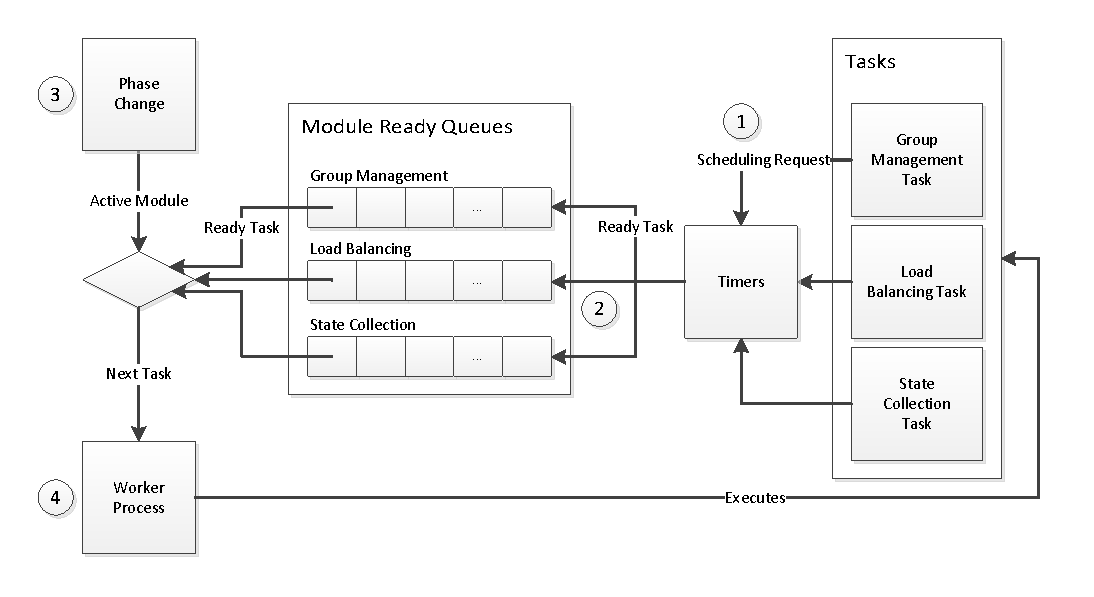
\includegraphics[width=1.0\textwidth]{RealTimeScheduler.pdf}
\captionsetup{singlelinecheck=off}
\caption[Real Time Scheduler]{The real time scheduler used a round robin approach to allot execution time to modules. 
\begin{enumerate}
    \item Modules requested that a task be executed by specifying a time in the future to execute a task.
          A timer was set to count down to the specified moment.
           Modules could place tasks immediately into the ready queue if the task could executed immediately.
    \item When the timer expires the task is placed into the ready queue.
    \item Modules were assigned periods of execution (called phases) which were a predetermined length.
          After the specified amount of time had passed, the module's phase ends and the next module in the schedule began to execute.
    \item The worker selected the next ready task for the active module from the ready queue and executed it.
          These tasks could also schedule other tasks to be run in the future.
\end{enumerate}
}
\label{fig:REALTIMESCHEDULER}
\end{figure}

Modules informed the scheduler of tasks they wish to perform.
The tasks could be scheduled for some point in the future, or scheduled to executed immediately.
When a tasks became ready was inserted into a ready queue for the module it was been scheduled for.

When that modules phase was active, tasks were pulled from the ready queue and executed.
When the phase was complete, the scheduler stopped pulling tasks from the previous module's queue and began pulling from the next module's queue.

This allowed enforcement of upper bound message delay.
Modules had a specific amount of processing time allotted.
Modules with messages that invoked responses typically required the responses to be received within the same phase.
Round numbers enforced that the message was sent within the same phase.

Modules were designed and allotted time to allow for parameters such as maximum query-response time (based on the latency between communicating processes).
This implied that a module that engaged in these activities has an upper-bound in latency before messages are considered lost.

\subsection{Group Management Algorithm}

The DGI uses the leader election algorithm, ``Invitation Election Algorithm,'' written by Garcia-Molina\cite{INVITATIONELECTION}.
Originally published in 1982, this algorithm provides a robust election  procedure that allows for transient partitions.
Transient partitions are formed when a faulty link between two or more clusters of \ac{DGI} causes the groups to divide temporarily.
These transient partitions merge when the link becomes more reliable.
The election algorithm allows for failures that disconnect two distinct sub-networks.
These sub networks are fully connected, but connectivity between the two sub-networks is limited by an unreliable link.

Since Garcia-Molina's original publication \cite{INVITATIONELECTION}, a large number of election algorithms have been created. 
Each algorithm is designed to be well-suited to the circumstances it will deployed in.
Specialized algorithms exist for wireless sensor networks\cite{LE-WSN-1}\cite{LE-WSN-2}, detecting failures in certain circumstances\cite{LE-SPECIALCIRCUMSTANCES-1}\cite{LE-SPECIALCIRCUMSTANCES-2}, and of course, transient partitions.
Work on leader elections has been incorporated into a variety of distributed frameworks: Isis\cite{ISISTOOLKIT}, Horus\cite{HORUSTOOLKIT}, Totem\cite{TOTEMTOOLKIT}, Transis\cite{TRANSISTOOLKIT}, and Spread\cite{SPREADTOOLKIT} all have methods for creating groups.
Despite this wide array of work, the fundamentals of leader election are consistent
across all work.
Processes arrive at a consensus of a single peer that coordinates the group.
Processes that fail are detected and removed from the group. 

The elected leader is responsible for making work assignments, and identifying and merging with other coordinators when they are found, as well as maintaining an up-to-date list of peers for the members of his group. 
Group members monitor the group leader by periodically checking if the group leader is still alive by sending a message. 
If the leader fails to respond, the querying nodes will enter a recovery state and operate alone until
they can identify another coordinator.
Therefore, a leader and each of the members maintain a set of processes which are currently reachable, a subset of all known processes in the system.

Leader election can also be classified as a failure detector\cite{LEADERELECTIONEVAL}.
Failure detectors are algorithms which detect the failure of processes within a system; they maintain a list of processes that they suspect have crashed.
This informal description gives the failure detector strong ties to the leader election process. 
The group management module maintains a list of suspected processes which can be determined from the set of all processes and the current membership.

The leader and the members have separate roles to play in the failure detection process.
Leaders use a periodic search to locate other leaders in order to merge groups.
This serves as a ping / response query for detecting failures within the system.
The member sends a query to its leader.
The member will only suspect the leader, and not the other processes in their group.

Using a leader election algorithm allows the \ac{FREEDM} system to autonomously reconfigure rapidly in the event of a failure.
Cyber components are tightly coupled with the physical components, and reaction to faults is not limited to faults originating in the cyber domain.
Processes automatically react to crash-stop failures, network issues, and power system faults.
The automatic reconfiguration allows processes to react immediately to issues, faster than a human operator, without relying on a central configuration point.
However, it is important the configuration a leader election supplies is one where the system can do viable work without causing physical faults like voltage collapse or blackouts\cite{HARINI}.

A state machine for the election portion of the election algorithm is shown in Figure \ref{fig:statemachine}.
In the normal state, the election algorithm regularly searches for other coordinators to join with.
When another coordinator is identified, all other processes will yield to their future coordinator.
The method of selecting which process becomes the coordinator of the new group differentiates the modified algorithm from other approaches.

\subsection{Power Management}

In this work we utilize the load balancing algorithm from \cite{LOADBALANCING}.
The load balancing algorithm performs work by managing power devices with a sequence of migrations\cite{HILTESTBED}.
In each migration, a sequence of message exchanges identify processes whose power devices are not sufficient to meet their local demand and other processes supply them with power by utilizing a shared bus.
To do this, first processes that cannot meet their demand announce their need to all other processes.
Processes with devices that exceed their demand offer their power to processes that announced their need.
These processes perform a three-way handshake.
At the end of the handshake, the two processes have issued commands to their attached devices to supply power from the shared bus and to draw power from the shared bus.
An example of how the power system is affected by migrations is depicted in Figure \ref{fig:good-migrations}.
In the chart, processes with net generation (generation $>$ 0) share power with processes with excess loads.
As processes with excess loads are satisfied, both supply processes and demand processes trend toward 0 net generation.

\begin{figure}
\centering
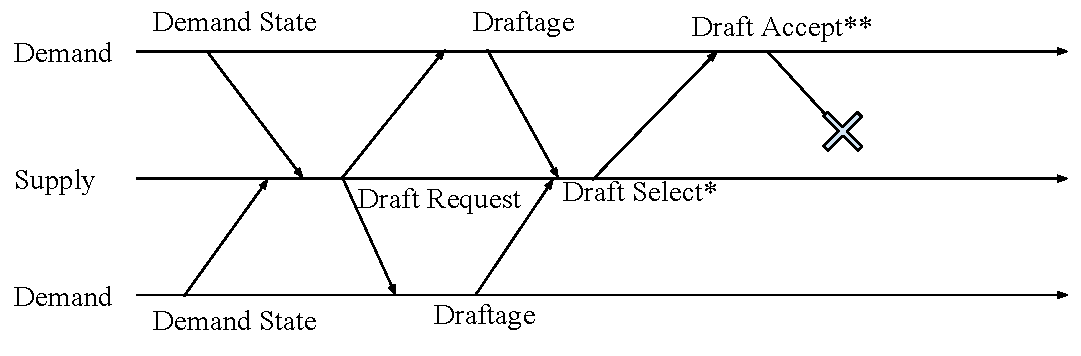
\includegraphics[width=0.95\textwidth]{FailedMigration1}
\caption{Example of a failed migration. (*) and (**) mark moments when power devices change state to complete the physical component of the migration. In this scenario, the message confirming the demand side made the physical is lost, leaving the supply node uncertain.}
\label{fig:failed-migration-1}
\end{figure}

\begin{figure}
\centering
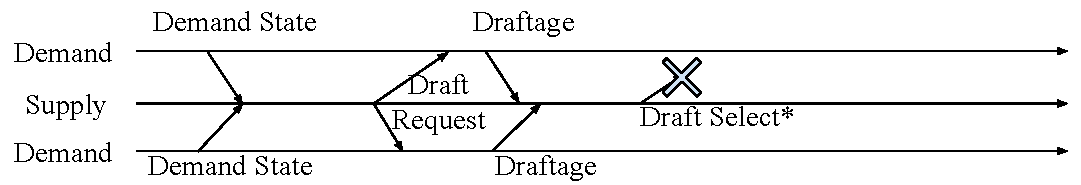
\includegraphics[width=0.95\textwidth]{FailedMigration2}
\caption{Example of a failed migration. (*) marks a moment when power devices change state to complete the physical component of the migration. In this scenario, the supply process changes its device state, but the demand process does not.}
\label{fig:failed-migration-2}
\end{figure}

\begin{figure}
\centering
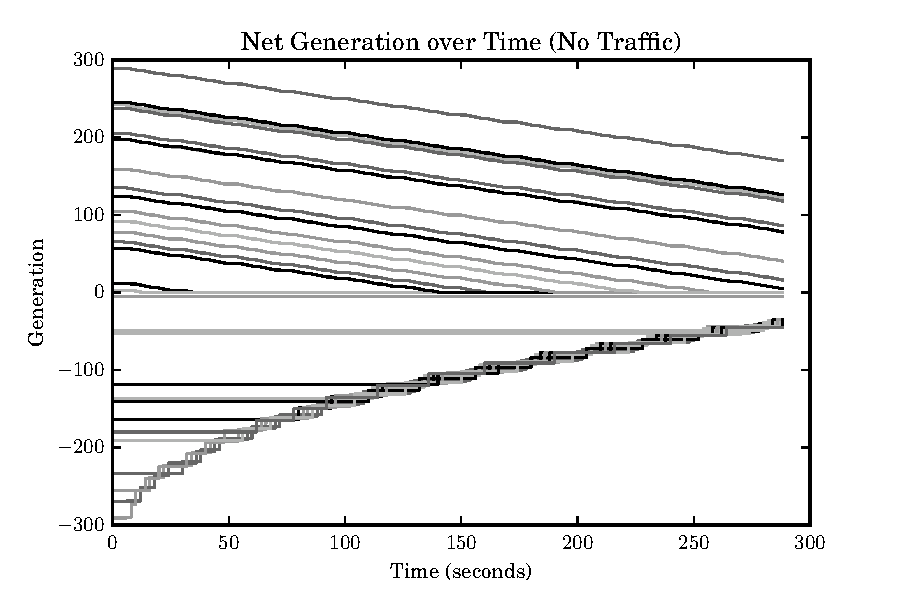
\includegraphics[width=0.75\textwidth]{c-migrations-no-traffic-all}
\caption{Each migration consumes excess generation capability and removes excess demand.}
\label{fig:good-migrations}
\end{figure}

The \ac{DGI} algorithms can tolerate packet loss and is implemented using UDP to pass messages between \ac{DGI} processes.
Effects of packet loss on the \ac{DGI}'s group management module have been explored in \cite{CRITIS2012} and \cite{JOURNAL}.
The load balancing algorithm can tolerate some message loss, but lost messages can cause migrations to only partially complete, which can cause instability in the physical network.
A failed migration is diagrammed in Figures \ref{fig:failed-migration-1} and \ref{fig:failed-migration-2}.
With this power migration algorithm, uncompensated actions may occur in the power system.
These actions can eventually lead to power instability through issues such as voltage collapse.
Additionally, the supply process may not always be certain if the second half of the action was completed or not.
If the ``Draft Accept'' message does not arrive from the demand process, the supply process cannot be certain of whether or not its ``Draft Select'' message was received.
If the supply process takes action to compensate by reversing the migration and the confirmation arrives later the system will also be driven towards instability because another process completed an uncompensated action.
Processes could confirm the number of failed migrations with a state collection technique.
It is therefore desirable to manage the processes to minimize the number failed migrations.


